\section{Results and Discussion}
\subsection{Binary--mixture confined between two walls}
Initially a binary--mixture of two fluids confined between two walls was studied, corresponding to the physical case of a liquid sandwiched between two plates.
The fluid was prepared as described in Section \ref{SystemPrep} at a pressure of $P^{*} = 0.1$ and temperatures of $T^{*} = 0.8$ and $T^{*} = 0.9$.
The confining walls were used as a piston to control the pressure.

\subsubsection{Using the Virial stress}\label{VirialStressPiston}
Once equilibrated, the simulations were run for $40 \times 10^{6}$ timesteps and the number--density and Virial stress--tensor were computed every timestep.
These values were then time-averaged to produce profiles for the number--density and $\sigma_{xx}(z^{*})$ expressed in terms of the scaled coordinate $z'$, as shown in Figures \ref{PisVirRho} and \ref{PisVirStress}. 

\FloatBarrier
\begin{figure*}[h]
\centering
\includegraphics[scale=0.8]{PisVirRho}
\caption{PisVirRho caption goes here.}
\label{PisVirRho}
\end{figure*}

\begin{figure*}[h]
\centering
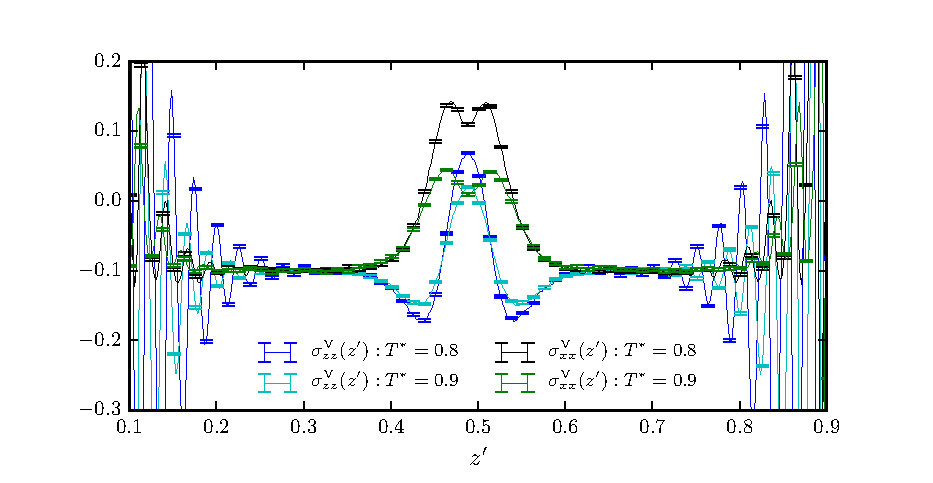
\includegraphics[scale=0.8]{PisVirStress}
\caption{PisVirStress caption goes here.}
\label{PisVirStress}
\end{figure*}

Both the density profile and the stress--profile show the expected features of a binary--mixture. 
There is a uniform density in the bulk of the fluid and an interfacial region of finite width where the density of one species falls sharply and the density of the other increases.
Close to the walls, there are large oscillations in the density that are a consequence of structural layering in the fluid close to the solid walls.
For the stress--profile, the bulk value for the tangential component is equal to $-P_{\mathrm{ext}}$, corresponding to the hydrostatic pressure of the fluid.
At the interface there is a peak in the tangential stress due to the anisotropy of the intermolecular forces in this region, this can be related to the interfacial tension.\cite{Marchand2011}

\FloatBarrier
The time--averaged values for the stress--tensor were then used to estimate the gradient of the stress--tensor with respect to temperature using Equation \ref{FinDiff}, as shown in Figure \ref{PisVirForce}.
This gradient also shows a peak at the interface of the two fluids, providing the origin of the  Marangoni force.
Importantly the gradient in the bulk of the fluid (far from both the interface and the walls) is zero within statistical error, ensuring there is no force acting in the bulk fluid.
In addition, there is an oscillating gradient at the surface of the wall which can be interpreted as a thermocapillary force.
Since we are only interested in simulating the Marangoni effect, these thermocapillary forces were ignored.
The central $1/3$ of the force profile was then used to create an artifical Marangoni force using a temperature gradient of $\partial T^{*} / \partial x^{*} = 0.001$ and Equation \ref{ForceStressTemp}.

\begin{figure*}[h]
\centering
\includegraphics[scale=0.8]{PisVirForce}
\caption{PisVirForce caption goes here.}
\label{PisVirForce}
\end{figure*}
\FloatBarrier

This artfical body force was then applied to an identical system prepared at $T^{*} = 0.85$.
A non-equilibrium simulation was run for $40 \times 10^{6}$ and the time--average of the x--component of the fluid velocity, $v^{*}_{x}(z')$, was computed.
The momenta of the walls in the $x$ and $y$ directions were fixed such that they provided a stationary reference point for the fluid.
As a result, the fluid shows non-slip boundary conditions and the walls act to hold the bulk fluid at rest.

\begin{figure*}[h]
\centering
\includegraphics[scale=0.8]{PisVirFlow}
\caption{PisVirFlow caption goes here.}
\label{PisVirFlow}
\end{figure*}
\FloatBarrier
The flow profile calculated for the fluid in this system is shown in Figure \ref{PisVirFlow}. 
There is a sharp negative peak at the interface of the two fluids indicating a Marangoni flow in the opposing direction to the temperature gradient.
Furthermore the flow decays linearly away from the interface, consistent with a Couette flow arising from shear--driven fluid motion.\cite{FluidMech}
There is also clearly a net flow of the fluid, suggesting a net force acting on the liquid.
The walls in the system act as a momentum sink, providing a friction force on the fluid which allows a steady--state flow to arise under the isolated effect of a temperature--gradient.
\FloatBarrier

\subsubsection{Comparing to the Irving--Kirkwood stress}
Figure \ref{PisVirRho} shows clearly that there are significant deviations in the fluid density at the interface and the walls and that the amount of deviation varies with temperature.
Because of the strong dependence of the Virial stress on the local density of the fluid, there is the potential for these changes to interfere with the measurement of the Marangoni force.
To verify the significance of these deviations, the stress--tensor was also calculated using the Irving--Kirkwood formula, since this does not depend on the local fluid density.

\begin{figure*}[h]
\centering
\includegraphics[scale=0.8]{PisIKStress}
\caption{PisIKStress}
\label{PisIKStress}
\end{figure*}
The fluids were prepared at $P^{*}=0.1$ and $T^{*}=0.8$ and $T^{*}=0.9$ as before.
Since the Irving--Kirkwood stress--tensor takes much longer to compute (see Section \ref{CalcStress}), the equilibrium simulations were only run for $1 \times 10^{6}$ timesteps, resulting in a greater amount of statistical error.
This produced the time--averaged stress--tensor profiles shown in \ref{PisIKStress}.
\FloatBarrier

\begin{figure*}[h]
\centering
\includegraphics[scale=0.8]{PisIKForce}
\caption{PisIKForce}
\label{PisIKForce}
\end{figure*}
The finite difference method was again used to calculate the gradient of this stress--tensor with respect to temperature and this is compared to the Virial result in Figure \ref{PisIKForce}.
Still focussing on only the central $1/3$ of the fluid, there is a good correspondence between the two gradient profiles and the interfacial peak occurs both across the same spatial region and with the same maximum value.
The most signifcant difference occurs directly at the interface, where there is a sharp reduction in the Irving--Kirkwood gradient.
This is probably a result of the reduction in density at the interface affecting the Virial stress--tensor more than the Irving--Kirkwood stress--tensor.
\FloatBarrier

\begin{figure*}[h]
\centering
\includegraphics[scale=0.8]{PisIKFlow}
\caption{PisIKFlow}
\label{PisIKFlow}
\end{figure*}
Using a temperature gradient of $\partial T^{*} / \partial x^{*} = 0.001$ to compute the Irving--Kirkwood aritifical body force, a non--equilibrium simulation at $T^{*} = 0.85$ was run for $40 \times 10^{6}$ timesteps.
This was compared to the flow profile calculated using the Virial force, as shown in Figure \ref{PisIKFlow}.
The flow profiles show a reasonably good correspondence, especially for the region $z' \leq 0.4$, although the profiles deviate for higher values of $z'$.
In particular the flow from the Irving--Kirkwood force is not as large directly at the interface, as a result of the reduction in the force at this point.
The velocity profile is also assymetric despite the symmetry of the system.
It is possible that this assymmetry is the result of an increase in the noise of the Irving--Kirkwood force relative to the Virial force, which in turn is a consequence of the shorter simulation time enforced by the high computational cost of the Irving--Kirkwood analysis.

\subsection{Binary--mixture periodic in 3-dimensions}
Equation \ref{NavierStokes} showed that the existence of a temperature gradient in the system should not be able to generate a net flow in the fluid. 
Levich discusses this further, describing how the interfacial flow must be accompanied by a back-flow in the bulk fluid.\cite{Levich}
In the case of the binary--mixture held between two walls, the stationary walls provide a momentum sink which allows a net flow to exist within the fluid.
To replicate the behaviour described by Levich, a system void of momentum sinks must be studied, for example a binary--mixture of two immiscible fluids with periodic boundary conditions in all dimensions.

 provides this, as shown on the left--hand side of Figure \ref{SetUp}.

This system, shown on the left--hand side of Figure \ref{SetUp}, was prepared as described in Section \ref{SystemPrep} with the parameters given in Section \ref{InteractionModel}.
The distance between consecutive interfaces was equal to $0.5 L_{z^{*}}$.
A Nos\'{e}--Hoover barostat and thermostat were used to control the pressure at $P^{*} = 0.1$ with temperatures of $T^{*}=0.8$ and $T^{*}=0.9$.

\subsubsection{Comparing the Virial and Irving--Kirkwood stress}
There is again an ambiguity over which stress--tensor should be used for computing the Marangoni force.
Initially, the equilibrated symmetric binary--mixture was simulated for $10 \times 10^{6}$ timesteps and the number--density, $\sigma^{\mathrm{V}}$ and $\sigma^{\mathrm{IK}}$ were computed.
As discussed before, the Irving--Kirkwood analysis was highly computationally expensive and this simulation length was the upper feasible limit.
\FloatBarrier

\begin{figure}[h]
\centering
\includegraphics[scale=0.8]{Period10Rho}
\caption{Period10Rho}
\label{Period10Rho}
\end{figure}
After this period, the density profile (plotted in Figure \ref{Period10Rho}) clearly showed a uniform density in the fluid bulk and a sharp interfacial region as expected.
However, the exact position of the interface had shifted slightly during the simulation and was no longer coincedent for the two temperatures.
To calculate the Marangoni force from the stress profile, this shift had to be manually removed by recentering the interfaces prior to computing the finite difference.
\FloatBarrier

\begin{figure}[h]
\centering
\includegraphics[scale=0.8]{Period10VirStress}
\caption{Period10VirStress}
\label{Period10VirStress}
\end{figure}

\begin{figure}[h]
\centering
\includegraphics[scale=0.8]{Period10IKStress}
\caption{Period10IKStress}
\label{Period10IKStress}
\end{figure}
The recentered Virial and Irving--Kirkwood stress profiles are plotted in Figure \ref{Period10VirStress} and Figure \ref{Period10IKStress} respectively.
As with the fluid confined between two walls, the bulk stress--tensor components are equal to $-P_{\mathrm{ext}}$, correpsonding to the hydrostatic fluid pressure.
There is a similar peak in both the Virial and Irving--Kirkwood stress at the interface.
The peaks also have the same maximum value for both stress--tensors, although the Irving--Kirkwood stress shows a stronger minimum directly at the interface.
As with the fluid confined between two walls, this is probably the result of a reduced density in the interfacial region.

\FloatBarrier
Using these stress profiles, the gradient of the stress with repsect to temperature was calculated from the finite difference approach.
For there to be no net force acting on the fluid, the gradient profile was adjusted by subtracting the average value from each value to ensure the intergral over all space was zero, as shown in Figure \ref{Period10Force}.
This replicated the effect of a momentum sink in the infinite periodic fluid, for example a distant boudning wall.

\begin{figure}[h]
\centering
\includegraphics[scale=0.8]{Period10Force}
\caption{Period10Force}
\label{Period10Force}
\end{figure}
The resulting gradient profile shows a similar peak at the interface to Figure \ref{PisIKForce}, with a similar maximum value suggesting that fixing the total force on the fluid to zero correctly adjusts the data to give a physically meaningful Marangoni force.
Again there is a reasonably good correspondence between the gradient calculated from the Irving--Kirkwood and Virial stress--tensors, although directly at the interface the magnitude of the Irving--Kirkwood peak is reduced.
Away from the interface there is a bulk gradient acting in the opposite direction to the interfacial peak, generating the expected back force away balancing the Marangoni force.
However the profile as a whole shows too much noise for the fine--structure to be determined and is not of a sufficient quality to be used in calculating an artificial body--force for a non--equilibrium simulation.

\subsubsection{Reducing the noise in the force--profile}
To generate a gradient profile with a sufficiently low level of nosie requires either a larger system size or a longer simulation time.
Both of these increase the computational cost of calculating the Irving--Kirkwood stress--tensor beyond a practical level and the Virial stress--tensor must be used.
Considering how similar the Virial and Irving--Kirkwood force profiles appear in Figure \ref{PisIKForce}, using the Virial stress--tensor does not create too much deviation from the more suitable Irving--Kirkwood stress--tensor whilst it would enable a much longer simulation time to achieved.
\FloatBarrier

\begin{figure}[h]
\centering
\includegraphics[scale=0.8]{Period30VirStress}
\caption{Period30VirStress}
\label{Period30VirStress}
\end{figure}

The reduced noise stress--profile was generated by running the equilibrium systems for $30 \times 10^{6}$ timesteps.
Recentering the interfaces generated the Virial stress profile shown in Figure \ref{Period30VirStress}.
For both temperatures the profiles show much less noise compared to Figure \ref{Period10VirStress}, especially in the bulk region, and the interfacial peaks are more symmetric.
\FloatBarrier

\begin{figure}[h]
\centering
\includegraphics[scale=0.8]{Period30VirForce}
\caption{Period30VirForce}
\label{Period30VirForce}
\end{figure}
Using this stress profile the gradient of the stress--tensor with respect to temperaturee was again computed using the finite difference and the average value subtracted to give the profile shown in Figure \ref{Period30VirForce}.
There is a dramatic reduction in the noise of this gradient profile compared to Figure \ref{Period10Force} and it clearly shows a sharp peak at the interface with an opposing gradient in the bulk regions.
\FloatBarrier

Using the gradients given in Figure \ref{Period30VirForce} and a temperature gradient of $\partial T^{*} / \partial x^{*} = 0.001$, an artifical body force was computed.
The body force was recentered to ensure that the peak corresponding to the Marangoni force aligned with the interfacial region at $T^{*} = 0.85$, and this was applied in a non--equilibrium simulation.
This simulation was run for $40 \times 10^{6}$ and the x--component of the velocity computed to yield the flow profile plotted in Figure \ref{Period30VirFlow}.

\begin{figure}[h]
\centering
\includegraphics[scale=0.8]{Period30VirFlow}
\caption{Period30VirFlow}
\label{Period30VirFlow}
\end{figure}

This flow profile still retains a lot of statistical noise, despite the simulation being run for a long timescale.
It would be practically difficult to reduce this noise further.
Moreover the average velocity (indicated the hashed line) is non--zero, implying that there is motion of the centre--of--mass during the simulation.
This centre--of--mass motion is occuring even though the force--profile has been recentered to give no net force overall.
It is likely that in the absence of a momentum sink for a system like this, it would be very difficult to completely remove this net flow without fixing the centre--of--mass artificially throughout the simulation.

Despite this, the relative motion across the fluid can still be considered and this does, to some extent, show a velocity peak at the interface (with $v < v_{\mathrm{COM}}$), corresponding to a Marangoni flow, and some evidence for the expected back flow in the bulk fluid (with $v > v_{\mathrm{COM}}$).
This result is, however, very ambiguous and there was insufficient time in the project to improve the non--equilibrium simulation further.

\subsection{The effect of surfactants}



